% ----------------------------------------------------------------------------
\chapter{Building Blocks of PTXdist} 		\label{chap:building-blocks}
% ----------------------------------------------------------------------------

\section*{The Big Picture}

PTXdist is good for basically two tasks: compiling stuff for an embedded
system, which means to compile components which go into the
\texttt{root/} directory of the PTXdist tree, and compiling tools which
are needed on the development host to build other code for the target. 

\begin{important}
The PTXdist manual does consequently talk about two computers you
usually work with: one is the \emph{development host} -- this is the
normal PC you work on. The development host needs a generic Linux
distribution (for example Debian, SuSE, RedHat or Mandrake).  The other
one is the \emph{embedded target}, sometimes also referenced as the
\emph{target}. The Target is usually an embedded device and may have
another processor architecture than your development host.
\end{important}

% -----------------
\begin{figure}[b]
	\centerline{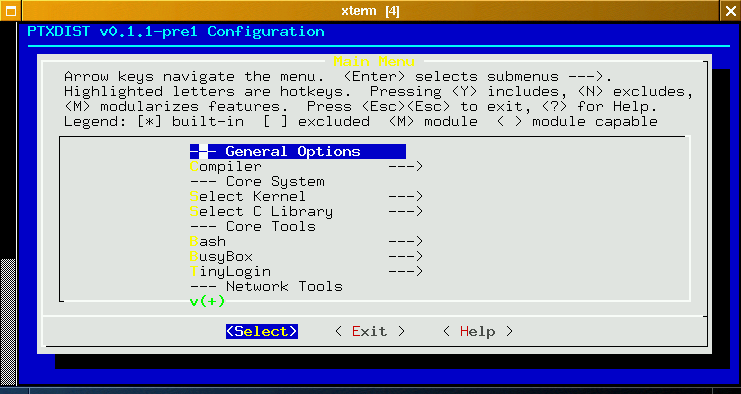
\includegraphics[width=0.99\textwidth]{figures/menuconfig}}
	\caption{
		KConfig in menuconfig mode: select what you want in your
		target. 	
		\label{fig:menuconfig}
	}
\end{figure}
% -----------------

Code for the host is being compiled with the distribution's native C
compiler (normally GCC), whereas you need a cross compiler to build code
for the target. We'll discuss later how you can get a cross compiler,
just in case you don't have one yet. 

Before we start digging deeper into PTXdist's internals let's have a
look at the building blocks the system consists of. The main building
blocks are: 

\begin{itemize}
\item The KConfig frontend (select what you want to have in your root
      filesystem), and
\item A set of Makefiles (rules which contain what has to be done).
\end{itemize}

The KConfig frontend is normally used by somebody who wants to configure
a \emph{selection} of programs which are later put into the root
filesystem of an embedded system; configuring mostly consists of
clicking on software components you want to install. Once you have a
working set of rules and a sane \emph{base} for your projects, you can
use the KConfig frontend to make your selection, without the need to do
further changes on a programming base. If you want to learn more about
how the KConfig system works, read section~\ref{chap:config-system}.
When you start working with PTXdist, somebody has normally already done
a more or less ready-to-use configuration. Check out which
configurations are available on your system: 

% -----------------
\begin{code}
robert@himalia:~/work/cvs-rsc/ptxdist> make configs

Available configs: 
[...]
i386-generic-glibc_config: 
[...]
toolchain-powerpc-405-linux_config:
toolchain-arm-linux-3.3.2_config:
toolchain-arm-linux-2.95_config:
[...]
\end{code} 
% -----------------

As you can see here, your PTXdist tree does currently have targets named
\emph{i386-generic-glibc\_config},
\emph{toolchain-powerpc-405-linux\_config},
\emph{toolchain-arm-linux-3.3.2\_config},
\emph{toolchain-arm-linux-2.95\_config}. According to the version you
are using you'll probably see more targets. The rules you see here are
so called \emph{config rules}. They all end in \emph{\_config} and their
task is to copy a pre-developed configuration into your toplevel
directory where it can be used to define what the next compiler run
generates. You can start one of these targets by running

\begin{code}
robert@himalia:~/ptxdist> make <foobar>_config  
\end{code}

while replacing \texttt{<foobar>} by the name of your configuration target.

% -----------------
\begin{important}
After you run \texttt{make <foobar>\_config} a predefined configuration
file, containing a set of to-be-installed applications, is copied into
your PTXdist directory. 

\vspace{1ex}

Don't forget to run \texttt{make oldconfig} now! This is necessary to
make a configuration ready for running and also checks if your
configuration is consistent to the config system of your currently used
PTXdist version. 
\end{important}
% -----------------

Now, you are ready for making it really happen. Until this moment, your
PTXdist tree does only contain what came from the archive; the next
steps the framework has to do is to get all the archives of the original
(\emph{upstream}) softare packets you need, extract them, prepare them
for compilation, put in the right configurations, run the cross compiler
(in case of tools for the target) or the host compiler (in case of host
tools) on them and, finally, install the compiled results into
appropriate places. 

We'll see later how all of these topics are done in detail, for now you
basically have to call \texttt{make world} to start the run. Take into
account that building a complete userland or toolchain does take some
time, so if your computer runs for several hours it might be just fine.

The result of the compiler run is a set of installed programs in their
respective places; if you have configured PTXdist for building a
userland you'll find your root filesystem in the \texttt{root/}
directory now, ready for being mounted to your target via NFS or being
flashed into some flash filesystem. 

If you ever want to cleanup your PTXdist tree, just enter \texttt{make
distclean} at the shell prompt. The distclean target brings your PTXdist
tree back into the state where you have started, which means that you
can safely start the whole thing again. If you don't want to lose your
configuration, enter \texttt{make clean} instead. This also cleans up
the build directories, but leaves the configuration intact. 

It is also possible to clean out single packets, which is helpful when
you want to change the configuration for one software component, but
don't want to recompile the whole system. We'll discuss later in
chapter~\ref{} how this is done. 

